\documentclass[conference,a4paper]{IEEEtran}

\usepackage{amsmath,amssymb}
\usepackage{booktabs}
\usepackage{balance}
\usepackage{cite}
\usepackage{graphicx}
\usepackage{siunitx}
\usepackage{tikz}
\usepackage{xcolor}
\usetikzlibrary{arrows.meta,positioning,fit}

\graphicspath{{figures/}}
\sisetup{detect-all}

\title{Decoupling-Oriented Coordination of Paralleled  VSGs With
Multi-Agent Reinforcement Learning}

\author{
\IEEEauthorblockN{Yuang Wei, Yixiao Wang, and Zhuang Xu}
\IEEEauthorblockA{
Department of Electrical and Electronic Engineering\\
University of Nottingham Ningbo China, Ningbo, China\\
John.XU@nottingham.edu.cn}
}

\begin{document}
\pagestyle{empty}
\maketitle
\renewcommand{\IEEEkeywordsname}{Keywords}

\begin{abstract}
Within the learned-policy canary bank, adaptive virtual inertia and damping can
satisfy decoupling endpoints while violating comparator-relative action limits.
This paper evaluates that distinction in a modified Kundur system with four
virtual synchronous generators (VSGs) after correcting the
device-to-system-base conversion. Four independent soft actor--critic agents
provide one way to adapt virtual inertia $M$ and damping $D$. We define a
complete guard-first contract that
separates common-frequency support, off-diagonal and differential response
energies, and physical and action no-harm checks. A deterministic direct-$M/D$
law selected on two development profiles passes the predefined deterministic
guard set on four prospectively fresh profiles at both \SI{6}{s} and
\SI{30}{s}. We then audit 208
frozen policies from a prospectively trained $2\times2\times2$ actor-source,
critic-source, and reward-access factorial with 26 paired training seeds. On a
separate four-profile \SI{30}{s} canary bank, 126 policies meet both aggregate
5\% endpoint-improvement targets relative to direct $M/D$. None passes the
complete contract: all 832 policy--profile blocks violate both registered
relative action-RMS and action-variation limits. At the separately reported
\SI{6}{s} and \SI{30}{s} horizons, none of four source-factor contrasts
establishes improvement above the 10\% materiality boundary after Holm control.
For these separate deterministic-fresh and learned-canary banks under the
registered parameter card, endpoint-only assessment qualifies policies that the
complete contract rejects; this does not imply a universal failure of
multi-agent reinforcement learning (MARL).
\end{abstract}

\begin{IEEEkeywords}
virtual synchronous generator, multi-agent reinforcement learning, virtual
inertia, frequency coordination, guard-first evaluation
\end{IEEEkeywords}

\section{Introduction}

Virtual synchronous generators (VSGs) reproduce swing-like behaviour in
converter controls and expose tunable inertia and damping
parameters~\cite{zhong2011synchronverters,darco2013vsm,wu2016smallsignal}.
When several units operate in parallel, fleet-average support and inter-unit
motion are different physical coordinates. Model-based consensus, mutual
damping, and parallel-VSM designs make that distinction explicit through their
feedback structure~\cite{liu2020consensus,shi2021restoration,fu2022mutual,
gao2024mutual,wang2024consensus,gonzalez2022parallel}.

Relevant precedents include distributed dynamic inertia--droop MARL for
paralleled VSGs~\cite{yang2023ddic}, single-VSG soft actor--critic $M/D$
tuning~\cite{lu2024sac}, MADDPG joint-$M/D$ control~\cite{zhang2024maddpg},
decentralized multi-VSG MARL~\cite{kang2025madrl}, and constraint-aware
power-system RL~\cite{tabas2022safe,shuai2025safe}. We inherit their broad
controller and learning elements. Our contribution is instead the
post-correction audit of a frozen family using separated development, fresh,
and canary banks, matched source interventions, split horizons, and
comparator-relative guards. It is neither a new learning algorithm nor a basis
for cross-system inference.
However, an aggregate reward or average-frequency trajectory cannot by itself
identify differential coordination. A favourable endpoint can also coexist
with large or rapidly varying commands, while actor, critic, and reward
information may change simultaneously in a nominal message/no-message
comparison. Reinforcement-learning seed variability further limits
small-sample conclusions~\cite{agarwal2021statistical}.

These issues became decisive in the present study. An audit found that the
original controller arithmetic and simulator runtime used different M/D bases.
After applying the device/system-base conversion exactly once, the previous
positive evidence was no longer admissible. A separate zero-adaptive-action
sensitivity bank also showed that a \SI{6}{s} window can miss the tail at high
inertia.
Accordingly, this paper treats unit correctness, horizon separation, and the
complete contract as part of the scientific question rather than
as implementation details.

Our goal is to determine whether corrected $M/D$-adaptive MARL provides
decoupling gains beyond a development-selected deterministic reference while satisfying
every registered guard. We use two signed
finite-window response energies, require per-profile validity and no-harm
checks before interpreting endpoints, and reserve the fresh evaluation bank
for the deterministic feasibility claim. Learned policies are judged on a
separate canary bank, so evidence is not transferred between controllers or
profile splits.

The evaluation combines a development-selected local-neighbour direct-$M/D$
law with a prospectively trained $2\times2\times2$ source/reward factorial.
Twenty-six
paired seeds support actor, critic, actor-by-critic, and critic-by-reward
contrasts. The registered \SI{6}{s} primary analysis and the evaluation-only
\SI{30}{s} tail sensitivity share frozen policies and are therefore reported
side by side but never pooled. Figure~\ref{fig:contract} summarizes the two
decision paths.

This paper makes four bounded contributions. First, Section~\ref{sec:contract}
specifies a corrected device/system-base action contract and separates common
and differential coordinates from empirical guard decisions. Second,
Sections~\ref{sec:protocol}--\ref{sec:results} establish a constructive
deterministic reference that passes four prospectively fresh \SI{30}{s}
profiles. Third, Section~\ref{sec:results} reports a complete 208-policy tail
audit showing that endpoint qualification and complete-contract satisfaction
can diverge: 126 policies meet both endpoint targets, while none satisfies the
complete contract. Fourth, Sections~\ref{sec:protocol}--\ref{sec:results} show that the
matched 26-seed factorial does not establish improvement above the 10\%
materiality boundary for any registered source contrast after multiplicity
control.

\begin{figure}[t]
\centering
\resizebox{\columnwidth}{!}{%
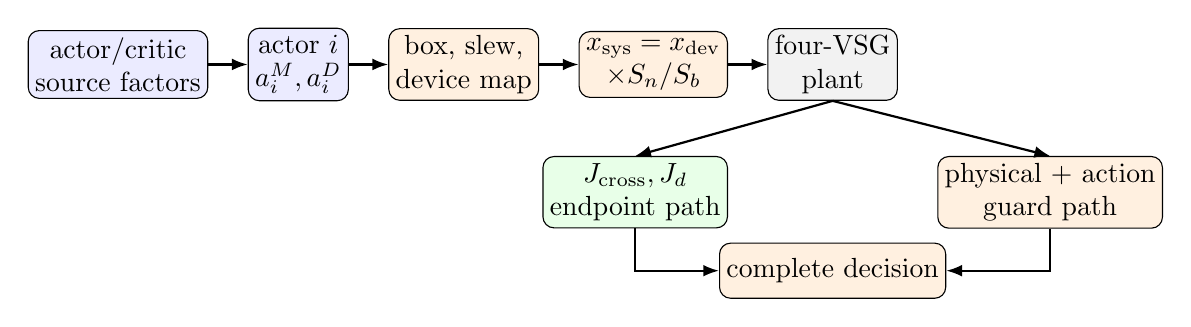
\begin{tikzpicture}[
  node distance=4mm and 5mm,
  box/.style={draw,rounded corners,minimum height=7mm,align=center,inner sep=2.5pt},
  input/.style={box,fill=blue!8},
  plant/.style={box,fill=gray!10},
  metric/.style={box,fill=green!9},
  guard/.style={box,fill=orange!12},
  arr/.style={-{Latex[length=2mm]},thick}
]
\node[input] (source) {actor/critic\\source factors};
\node[input,right=of source] (actor) {actor $i$\\$a_i^M,a_i^D$};
\node[guard,right=of actor] (map) {box, slew,\\device map};
\node[guard,right=of map] (base) {$x_{\rm sys}=x_{\rm dev}$\\$\times S_n/S_b$};
\node[plant,right=of base] (plant) {four-VSG\\plant};
\draw[arr] (source)--(actor);
\draw[arr] (actor)--(map);
\draw[arr] (map)--(base);
\draw[arr] (base)--(plant);
\node[metric,below left=7mm and 5mm of plant] (endpoints) {$J_{\rm cross},J_d$\\endpoint path};
\node[guard,below right=7mm and 5mm of plant] (guards) {physical + action\\guard path};
\node[guard,below=18mm of plant] (decision) {complete decision};
\draw[arr] (plant.south)--(endpoints.north);
\draw[arr] (plant.south)--(guards.north);
\draw[arr] (endpoints.south) |- (decision.west);
\draw[arr] (guards.south) |- (decision.east);
\end{tikzpicture}}
\caption{Corrected guard-first evaluation. Per-VSG actions are decoded on the
device base and converted exactly once at the simulator boundary. Endpoint
improvement is interpreted only after the physical and action guard path
passes.}
\label{fig:contract}
\end{figure}

\section{Coordination Object and Guard-First Contract}
\label{sec:contract}

\subsection{Corrected physical and action object}

We consider four controlled VSGs in a modified Kundur two-area system. Their
angle and frequency states follow
\begin{equation}
\dot{\delta}_i=2\pi f_n(\omega_i-1),\qquad
M_i^{\mathrm{sys}}\dot{\omega}_i
=\tau_{m,i}-\tau_{e,i}-D_i^{\mathrm{sys}}(\omega_i-1),
\label{eq:swing}
\end{equation}
where reported physical frequency uses the Kundur $f_n=\SI{60}{Hz}$ base.
Equation~\eqref{eq:swing} fixes the physical state convention used below.
Controller arithmetic is performed on the device base, whereas ANDES stores
runtime parameters on the system base~\cite{cui2021andes}. Each boundary
crossing therefore applies exactly one conversion,
\begin{equation}
x_i^{\mathrm{sys}}=x_i^{\mathrm{dev}}\frac{S_{n,i}}{S_b},
\qquad x\in\{M,D\},\qquad M=2H .
\label{eq:base_conversion}
\end{equation}
The registered parameter card uses $S_b=\SI{100}{MVA}$,
$S_{n,i}=\SI{200}{MVA}$, $H_0^{\mathrm{dev}}=\SI{100}{s}$,
$M_0^{\mathrm{dev}}=\SI{200}{s}$, and $D_0^{\mathrm{dev}}=100$.
These values define the corrected project calibration; they do not reconstruct
an unspecified baseline from prior literature.
% Evidence: R478/CLM-1485 and md_parameter_card_20260824.json.

At each \SI{0.2}{s} control instant, controller $i$ produces a normalized
target $\bar a_i$. Let $\Pi_c(x)=\min\{c,\max\{-c,x\}\}$ componentwise. With
$a^{\rm exec}_i[-1]=0$, the common projection is
\begin{equation}
\begin{aligned}
a_i^{\rm amp}[k]&=\Pi_1(\bar a_i[k]),\\
a_i^{\rm exec}[k]&=\Pi_1\!\left(a_i^{\rm exec}[k-1]\right.\\
&\quad\left.+\Pi_{0.25}\!\left(a_i^{\rm amp}[k]
-a_i^{\rm exec}[k-1]\right)\right).
\end{aligned}
\label{eq:projection}
\end{equation}
The projected components then enter the decoder
\begin{equation}
\begin{aligned}
q(a)&=\begin{cases}600a,&a\geq0,\\200a,&a<0,\end{cases}\\
M_i^{\mathrm{dev}}[k]&=\max\{20,M_{i,0}^{\mathrm{dev}}+q(a_i^{M,{\rm exec}}[k])\},\\
D_i^{\mathrm{dev}}[k]&=\max\{10,D_{i,0}^{\mathrm{dev}}+q(a_i^{D,{\rm exec}}[k])\}.
\end{aligned}
\label{eq:action_map}
\end{equation}
After \eqref{eq:base_conversion}, each decoded target is linearly applied over
five simulator substeps from the preceding runtime readback. Thus, projection
precedes decoding; no learned action directly injects active power.
% Evidence: md_parameter_card_20260824.json action_map, clamps, and slew.

\subsection{Common--differential endpoints}

Let $\Delta f\in\mathbb{R}^{4}$ be the physical VSG-frequency deviations. We
use $z_c=\mathbf{1}^{\top}\Delta f/4$ and
\begin{equation}
z_d=T_d\Delta f,\quad
T_d=\begin{bmatrix}
1/2&1/2&-1/2&-1/2\\
1/\sqrt{2}&-1/\sqrt{2}&0&0\\
0&0&1/\sqrt{2}&-1/\sqrt{2}
\end{bmatrix}.
\label{eq:coordinates}
\end{equation}
The coordinates in \eqref{eq:coordinates} are registered arithmetic
coordinates, not identified modal coordinates, and $z_c$ is not an
inertia-weighted centre-of-inertia frequency.

For probe type $k\in\{c,d,\ell\}$, let
$\varepsilon_c=\varepsilon_d=q$ and $\varepsilon_\ell=\ell$ for that profile.
The odd response of a matched signed pair is
$\widetilde f_k[n]=(\Delta f_k^+[n]-\Delta f_k^-[n])/2$. With
$z_{c,k}=\mathbf{1}^{\top}\widetilde f_k/4$ and
$z_{d,k}=T_d\widetilde f_k$, the lower-is-better endpoints are
\begin{align}
J_{\mathrm{cross}}={}&
\frac{\Delta t}{\varepsilon_c^2}
\sum_{n=1}^{N_T}\frac{\|z_{d,c}[n]\|_2^2}{3}
+\frac{\Delta t}{\varepsilon_d^2}
\sum_{n=1}^{N_T}z_{c,d}^2[n], \label{eq:jcross}\\
J_d={}&
\sum_{k\in\{c,d,\ell\}}
\frac{\Delta t}{\varepsilon_k^2}
\sum_{n=1}^{N_T}\frac{\|z_{d,k}[n]\|_2^2}{3}.
\label{eq:jd}
\end{align}
The endpoints in \eqref{eq:jcross} and \eqref{eq:jd} use
$\Delta t=\SI{0.2}{s}$ and $N_T=T/\Delta t$ for the separately
reported $T=\SI{6}{s}$ and $T=\SI{30}{s}$ horizons. The quantities are
discrete response energies, not joules, storage functions, or Lyapunov
functions.

\subsection{Guard-first decisions}

The following checks define the \emph{complete guard-first contract}, shortened
to \emph{complete contract} below. Endpoint improvement is interpreted only
after trajectory validity, actuator
mapping, normalized box and slew limits, common-frequency integral, worst-unit
peak, RoCoF, command stress, saturation, and action-nondegeneracy checks.
For learned policies, the three frequency quantities must be no worse than
103\% of the same-profile deterministic reference; executed-action RMS and
total variation must be no worse than 110\%; saturation fraction must be at
most 0.05; and the registered variation and per-VSG-dispersion floors are
$10^{-6}$.
These limits were registered before the canary outcomes and imported by hash.
They are empirical comparator-relative tolerances to prevent endpoint gains
from masking frequency (3\%) or command-stress (10\%) degradation, not
industry- or hardware-calibrated limits. Because the sealed audit stores
qualification rather than action-ratio margins, rejection is limited to these
exact thresholds; neighbouring-cutoff sensitivity is unassessed.

A learned policy passes the complete contract only when every one
of four canary profiles passes all per-profile guards and the equal-weight
aggregate ratios of both $J_{\mathrm{cross}}$ and $J_d$ are at most 0.95
relative to the deterministic controller. Deterministic fresh-bank feasibility
uses a predefined zero-action-referenced version of these checks, including
3\% frequency no-harm limits and the same mapping, bound, slew, saturation,
nonconstant-action, and per-VSG-dispersion checks. Its endpoint ratios are
descriptive report lines rather than gate inputs. Training reward cannot
override either decision. This follows the broader separation between
optimization penalties and verified closed-loop constraints
in safe power-system reinforcement learning~\cite{tabas2022safe,shuai2025safe}.
These empirical guards are not stability or safety certificates.
% Evidence: R484 plan lines 87--102 and R484/CLM-1520.

\section{Corrected Adaptive MARL Evaluation}
\label{sec:protocol}

\subsection{Profiles and deterministic reference}

Each profile contains common, differential, and localized probes, each with
positive and negative signs, giving six signed scenarios. The frozen learner
retains its registered \SI{50}{Hz} controller scaling, whereas physical
frequency endpoints use the \SI{60}{Hz} plant base. The parameter-card anchor
is $H_0=\SI{100}{s}$ unless overridden by the registered profile vectors in
Table~\ref{tab:profiles}. For a profile with magnitudes $q$ and $\ell$, the common
probe applies $\pm q/4$ at each of four loads, the differential probe applies
$\pm q/4$ to PQ0/PQ1 and $\mp q/4$ to B14/B15, and the localized probe applies
$\pm\ell$ at the listed load. Table~\ref{tab:profiles} gives every profile used
for selection, training, or evaluation.

\begin{table*}[t]
\caption{Registered profile cards. $M_0,D_0$ are four-VSG device-base vectors;
$P_{14},P_{15},q,\ell$ are system-p.u. active-power quantities. D denotes
deterministic development, T learner training, F deterministic fresh evaluation,
and C learned-policy canary evaluation.}
\label{tab:profiles}
\centering
\scriptsize
\setlength{\tabcolsep}{3.0pt}
\begin{tabular}{@{}clllrrrrl@{}}
\toprule
ID & Role & $M_0$ & $D_0$ & $P_{14}$ & $P_{15}$ & $q$ & $\ell$ & Local load\\
\midrule
D1 & development & [230,220,190,250] & [70,80,150,110]  & 1.92 & 0.42 & 0.70 & 1.05 & B14\\
D2 & development & [180,140,150,210] & [140,100,70,50]  & 2.08 & 0.52 & 1.15 & 0.95 & B15\\
T1 & training & [150,250,170,230] & [60,140,80,120] & 2.24 & 0.42 & 0.85 & 0.95 & PQ1\\
T2 & training & [230,150,250,170] & [120,60,140,80] & 2.02 & 0.66 & 1.05 & 1.15 & B15\\
T3 & training & [210,190,160,240] & [130,70,110,90] & 2.42 & 0.14 & 0.75 & 0.85 & PQ0\\
T4 & training & [240,160,190,210] & [90,110,70,130] & 2.12 & 0.54 & 0.95 & 1.05 & B14\\
F1 & fresh eval. & [190,200,140,160] & [110,120,130,70] & 1.92 & 0.64 & 1.15 & 0.95 & PQ1\\
F2 & fresh eval. & [230,140,250,150] & [60,90,70,110]   & 2.04 & 0.58 & 1.00 & 1.20 & PQ0\\
F3 & fresh eval. & [200,170,250,140] & [60,80,70,140]   & 2.40 & 0.36 & 0.90 & 0.85 & B14\\
F4 & fresh eval. & [190,150,170,220] & [120,130,80,110] & 2.58 & 0.28 & 0.75 & 0.90 & PQ0\\
C1 & canary eval. & [140,260,200,220] & [50,150,90,130] & 2.56 & 0.34 & 0.90 & 1.00 & PQ0\\
C2 & canary eval. & [260,140,220,200] & [150,50,130,90] & 2.06 & 0.26 & 0.80 & 0.90 & B14\\
C3 & canary eval. & [180,240,150,210] & [70,130,60,110] & 1.96 & 0.64 & 1.00 & 1.10 & B15\\
C4 & canary eval. & [220,200,260,140] & [110,90,150,50] & 2.32 & 0.46 & 1.10 & 1.20 & PQ1\\
\bottomrule
\end{tabular}
\end{table*}

Learner episodes cycle deterministically through the 24 T1--T4 signed
profile--scenario combinations. F1--F4 are reserved for deterministic
evaluation, and C1--C4 are reserved for learned-policy evaluation.

A separate zero-action screen showed that the worst-unit peak absolute
frequency deviation over \SI{6}{s} changed by 89.8\%--92.9\% at
$H_0=\SI{10}{s}$ and by
$-34.6\%$--$-34.3\%$ at $H_0=\SI{300}{s}$ relative to the anchor; at high
inertia this peak could occur after \SI{6}{s}. We therefore add a separate
\SI{30}{s} tail without claiming cross-$H$ controller robustness.
% Evidence: R480/CLM-1500; R484 frozen setup.

The deterministic family contains zero action and nine local-neighbour
direct-$M/D$ laws with $(k_M,k_D)\in\{0.5,1,2\}^2$. Let $\mathcal N_i$ contain
agent $i$'s two ring neighbours. The direct law uses dimensionless,
physical-\SI{60}{Hz}-calibrated features
$\phi_i=2\pi60(\omega_i-1)/3$ and $\rho_i=2\pi60\dot\omega_i/5$; equivalently,
it multiplies the registered learner observation's six frequency/RoCoF slots by
$60/50$, while learned policies retain the registered \SI{50}{Hz} scaling.
Before the common projection and decoder, each direct law forms
\begin{align}
\sigma_i={}&|\phi_i|+|\rho_i|,\nonumber\\
\bar a_i^M={}&\tanh\!\left[k_M\!\left(\sigma_i-
\frac{1}{2}\sum_{j\in\mathcal N_i}\sigma_j\right)\right],\nonumber\\
\bar a_i^D={}&\tanh\!\left[k_D\!\left(|\phi_i|+
\frac{1}{2}\sum_{j\in\mathcal N_i}
(|\phi_i-\phi_j|+|\rho_i-\rho_j|)\right)\right].
\label{eq:direct_md}
\end{align}
A candidate is development-eligible only if all runs are valid, common-frequency
no-harm checks pass, and saturation is at most 0.05. Among eligible candidates,
a frozen ascending lexicographic rule minimizes the worse of the two D1--D2
aggregate endpoint ratios to zero action, their sum, summed action RMS, and
finally the arm-identifier string as an exact tie-breaker. It selected
$(k_M,k_D)=(2,2)$. We then
evaluated the selected law on F1--F4 without reselection. The same controller
and profiles were rerun to \SI{30}{s}; the \SI{6}{s} and \SI{30}{s}
observations are not counted as eight independent profiles.
% Evidence: R481/CLM-1505 and R484/CLM-1520.

\subsection{Prospectively trained source factorial}

The MARL family contains four independent per-VSG soft actor--critic
learners~\cite{haarnoja2018sac}. It is neither parameter-shared nor a
joint-critic centralized-training/decentralized-execution method such as
MADDPG~\cite{lowe2017maddpg}. Each local state contains active power,
frequency, RoCoF, two ring-neighbour frequency/RoCoF pairs, and the agent's
previously executed two-component action. Specifically,
$o_i=[P_i/2,\delta\omega_i/3,\dot{\delta\omega}_i/5,
\delta\omega_{j_1}/3,\delta\omega_{j_2}/3,
\dot{\delta\omega}_{j_1}/5,\dot{\delta\omega}_{j_2}/5]$ and
$s_i=[o_i,a^{\rm exec}_{i,t-1}]\in\mathbb R^9$. The Gaussian--tanh actor and
twin-Q critic each use four 128-unit ReLU hidden layers. Adam uses a learning rate of
$3\times10^{-4}$, with $\gamma=0.99$, target-update rate $\tau=0.005$, replay
capacity 10,000, batch size 256, target entropy $-2$, automatic entropy
coefficient in $[0.005,5]$, and unit gradient-norm clipping. Once replay holds
256 transitions, one update follows each environment step. Projected executed
actions enter the current, target, and actor Q paths.

Actor and critic observation views are intervened separately. Source $N$ is
the authentic same-time neighbour tuple. For the frozen circular donor map
$\pi(i)=(i+1)\bmod4$, placebo source $P$ keeps the three recipient-local
entries and takes the four neighbour entries from donor row $\pi(i)$:
$P_i=[N_{i0},N_{i1},N_{i2},N_{\pi(i)3},N_{\pi(i)4},N_{\pi(i)5},N_{\pi(i)6}]$.
Thus, recipients 0--3 use donor rows 1, 2, 3, 0.
Thus, $N$ versus $P$ is a same-time total source intervention, not an isolated
semantic-information effect. The per-agent training reward is
\begin{equation}
r_i=100r_{f,i}+50r_{\mathrm{abs},i}+0.0056r_H+0.0056r_D,
\label{eq:reward}
\end{equation}
where reward access $r\in\{0,1\}$,
$\Delta f_i^{\rm Hz}=3o_i[1]/(2\pi)$,
$\overline{\Delta f}_i=(\Delta f_i^{\rm Hz}
+r\sum_{j\in\mathcal N_i}\Delta f_j^{\rm Hz})/(1+2r)$, and
\begin{align}
r_{f,i}&=-(\Delta f_i^{\rm Hz}-\overline{\Delta f}_i)^2
-r\!\sum_{j\in\mathcal N_i}(\Delta f_j^{\rm Hz}-\overline{\Delta f}_i)^2,
\nonumber\\
r_{{\rm abs},i}&=-(\Delta f_i^{\rm Hz})^2,\nonumber\\
r_H&=-\left(\frac{\frac14\sum_m\Delta M_m}{600}\right)^2,
\quad r_D=-\left(\frac{\frac14\sum_m\Delta D_m}{600}\right)^2.
\label{eq:reward_terms}
\end{align}
Reward access switches only the neighbour-dependent terms; reward is never used
by the evaluation contract.

The experiment crosses actor source $\{N,P\}$, critic source $\{N,P\}$, and
reward access $\{0,1\}$; the last factor switches only the registered
neighbour-dependent reward terms. Twenty-six matched seeds, 501--526, populate
all eight arms for 208 newly trained cells. Policies from earlier pilot training
do not enter the inference. Each cell could run from 30,000 to 43,200
interaction steps, with checks comparing adjacent 2,000-update windows and
termination allowed only after three consecutive qualifying checks. A check
requires finite loss, entropy-coefficient, and actor-gradient histories. It also
requires actor- and critic-loss median absolute magnitudes within a factor 1.10
across adjacent windows; entropy-coefficient medians either both at most
$1.01(0.005)$ or within a factor 1.05; an actor-gradient median absolute
magnitude of at least $10^{-6}$ and window ratio within a factor 1.25; zero
time-domain-simulation failures; and at most 2\% drift on a fixed-state
deterministic-action probe. The fixed 21,600-step midpoint and stopping-rule
final checkpoints define 16 registered arm-by-checkpoint evaluation batches;
the final checkpoint and \SI{6}{s} $J_d$ form the primary factorial.
% Evidence: R483 frozen setup and CLM-1515.

For statistical reconstruction, let $y_{acrps}=\log L_{acrps}$, where $L$ is
the positive final-checkpoint $J_d$ for actor source $a$, critic source $c$,
reward access $r$, profile $p$, and seed $s$. With angle brackets denoting
equal weighting over the displayed nuisance indices, the four within-seed
estimands are
\begin{align}
d_s^A={}&\langle y_{Pcrps}-y_{Ncrps}\rangle_{c,r,p},\nonumber\\
d_s^C={}&\langle y_{aPrps}-y_{aNrps}\rangle_{a,r,p},\nonumber\\
d_s^{AC}={}&\langle y_{PNrps}-y_{NNrps}
-y_{PPrps}+y_{NPrps}\rangle_{r,p},\nonumber\\
d_s^{CR}={}&\langle y_{aP1ps}-y_{aN1ps}
-y_{aP0ps}+y_{aN0ps}\rangle_{a,p}.
\label{eq:contrasts}
\end{align}
Thus, positive main effects mean lower loss under authentic source $N$;
positive interactions follow the registered ratio-of-ratios direction. The 26
matched seeds, not profiles or trajectories, are the inferential units. Tests
centre \eqref{eq:contrasts} at the materiality boundary $\log(1.10)$. The exact
upper-tail Wilcoxon test is primary when centred differences contain neither
zeros nor tied absolute ranks and have absolute Fisher--Pearson skewness at
most 1; otherwise, a prespecified one-million-draw upper-tail sign-flip mean
test (seed 20260825) is primary. All four observed contrasts passed the exact
route; sign flipping remains a sensitivity. Holm control covers the four-test
family~\cite{holm1979simple}.
Table~\ref{tab:source_effects} descriptively reports
$\Delta_{\rm geo}=100\{\exp(\langle d_s\rangle_s)-1\}\%$, positive toward an
authentic-source benefit. The signed-rank test targets a rank-based location
shift, not this mean-log summary; its $p$ values are not an interval for
$\Delta_{\rm geo}$.

The tail audit freezes all 208 final policies and introduces no training,
tuning, checkpoint selection, or parameter change. Policies run for 150 steps
on four registered canary profiles; learned policies never run on the fresh
bank. The complete inventory contains 16/16 valid shards, 848/848 profile
blocks (832 learned-policy and 16 zero/direct-$M/D$ reference blocks), and
5,088/5,088 valid trajectories. The \SI{30}{s} source calculation
uses the same 26 paired seeds and is a sensitivity analysis, not an independent
replication of the \SI{6}{s} primary analysis.
% Evidence: R484 identity, frozen setup, O1, and limits.

\section{Results}
\label{sec:results}

Figures~\ref{fig:direct_horizon} and~\ref{fig:learned_tradeoff} report,
respectively, deterministic fresh-bank feasibility and learned canary-bank
endpoint and contract decisions; the evidence objects remain non-pooled.

\begin{figure}[!b]
\centering
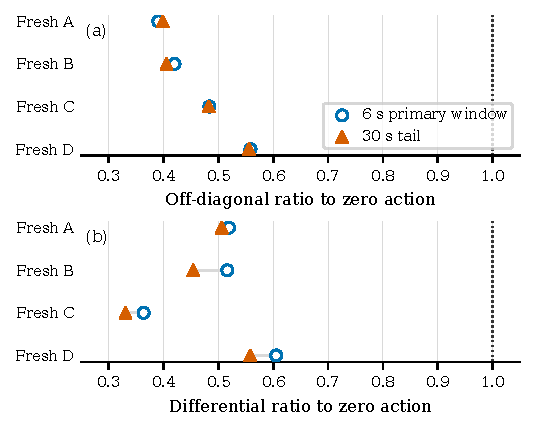
\includegraphics[width=0.995\columnwidth]{direct_md_fresh_horizon.pdf}
\caption{The development-selected direct-$M/D$ law remains guard-valid on all
four prospectively fresh profiles at the registered \SI{6}{s} window and the
separate \SI{30}{s} tail. Lines connect the same profile across horizons; the
dotted line is zero-action parity. Ratios are descriptive report lines, not
deterministic-guard inputs.}
\label{fig:direct_horizon}
\end{figure}
% Evidence: R481 phase1a_gate and R484 deterministic_fresh_tail.

\begin{figure*}[!t]
\centering
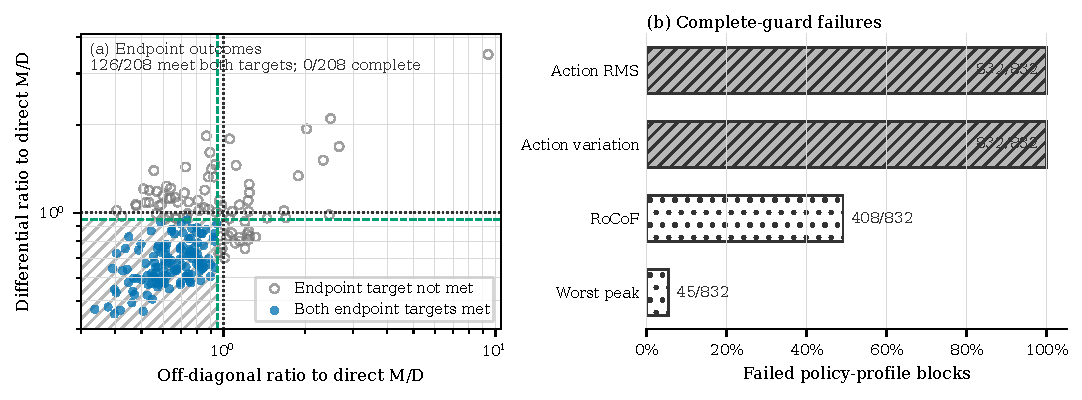
\includegraphics[width=\textwidth]{learned_contract_tradeoff.pdf}
\caption{Endpoint improvement is not complete-contract satisfaction.
(a) Each point is one frozen policy on the equal-weight four-profile canary
aggregate; lower is better. Green dashed lines mark the two 0.95 endpoint
targets, black dotted lines mark parity, and hatching marks their joint target
region. (b) Exact failure counts across all 832 policy--profile blocks.
Although 126/208 policies meet both aggregate endpoint targets, 0/208 passes
the complete contract because every block violates both comparator-relative
action-stress limits.}
\label{fig:learned_tradeoff}
\end{figure*}
% Evidence: R484 learned_guard policy_decisions and per_profile_blocks.

\subsection{Deterministic reference feasibility}

The corrected mapping and trajectory-integrity checks pass. The selected
direct-$M/D$ controller also passes the predefined deterministic guard on all
four prospectively fresh profiles at \SI{6}{s} and, separately, at
\SI{30}{s}. At the latter horizon, the off-diagonal ratios to zero
action range from 0.3987 to 0.5559, and the differential ratios range from
0.3307 to 0.5580. The plotted ratios describe response reduction; they are not
deterministic-guard inputs.

Direct $M/D$ also passes 4/4 canary profiles, but that result is descriptive
and used only to validate the learned-policy reference. It is not pooled with
the fresh result.

\subsection{Endpoint improvement does not satisfy the complete contract}

The learned-policy audit yields a sharp endpoint/action-limit separation.
Although 126/208 policies reduce both equal-weight aggregate endpoints by at
least 5\% relative to direct $M/D$, no policy passes the complete contract and
no policy passes the full per-profile guard set on even one canary profile.
All 832/832 learned
policy--profile blocks violate both registered relative action-stress limits.
Additionally, 408 blocks fail RoCoF no-harm and 45 fail worst-unit-peak
no-harm, while all common-frequency-integral checks pass.

The result is therefore not an absence of endpoint movement. Rather, the
endpoint reductions coexist with command stress, and for some blocks with
frequency stress, beyond the frozen comparator-relative allowances. Those
relative limits are not absolute hardware-energy bounds.

\subsection{Registered source effects}

Every one of the 208 training cells reached 43,200 steps without satisfying
the registered convergence certificate. Adaptive stopping therefore saved no
training time, but this neither invalidates the completed evaluations nor
proves divergence. Table~\ref{tab:source_effects} reports the four contrasts at
the two non-pooled horizons. No contrast establishes improvement above the
10\% materiality boundary after Holm control.

\begin{table}[t]
\caption{Non-pooled descriptive source estimates and Holm-adjusted tests}
\label{tab:source_effects}
\centering
\scriptsize
\setlength{\tabcolsep}{2.6pt}
\begin{tabular}{@{}lrrrr@{}}
\toprule
& \multicolumn{2}{c}{\SI{6}{s} primary}
& \multicolumn{2}{c}{\SI{30}{s} sensitivity}\\
Effect & $\Delta_{\rm geo}$ & $p_{\rm Holm}$
       & $\Delta_{\rm geo}$ & $p_{\rm Holm}$\\
\midrule
Actor main           & $-3.50\%$  & 1.0000 & $-4.99\%$  & 1.0000\\
Critic main          & $+5.20\%$  & 1.0000 & $+9.67\%$  & 1.0000\\
Actor$\times$critic  & $+21.81\%$ & 0.1187 & $+28.15\%$ & 0.0815\\
Critic$\times$reward & $+4.56\%$  & 1.0000 & $-5.37\%$  & 1.0000\\
\bottomrule
\end{tabular}
\end{table}
% Evidence: R483 factorial_materiality_tests; R484 tail_factorial_sensitivity.

The actor-by-critic point estimates cross the 10\% materiality boundary, but
their raw one-sided $p$ values of 0.02968 and 0.02037 become 0.1187 and 0.0815
after Holm correction. They are therefore hypothesis-generating rather than
confirmed material interactions. Failure to establish a material interaction
does not establish a zero effect or equivalence.

\section{Discussion and Limitations}
\label{sec:discussion}

The deterministic result shows that the corrected direct-$M/D$ feasible set is
nonempty within the registered finite bank. The learned result identifies a
different boundary: endpoint-only assessment would qualify 126/208 policies,
whereas the complete contract qualifies 0/208. The central
lesson is not that the tested learners cannot reduce differential response,
but that the policy-level endpoint and block-level action decisions separate:
126 policies meet both aggregate endpoint targets, while all 832 blocks violate
both frozen relative action allowances. This establishes tested-bank
co-occurrence, not a causal exchange between endpoint reduction and stress for
each qualified policy.

Earlier RL-based VSG studies use different plants, learners, rewards, and
validation objectives~\cite{yang2023ddic,lu2024sac,zhang2024maddpg,
kang2025madrl}. The combined unit-corrected, bank- and horizon-separated,
guard-first audit is the bounded distinction here. Its findings neither confirm
nor contradict their controller improvements; they delimit this tested contract.

The source factorial adds a second boundary. Neither horizon establishes a
registered source effect above 10\% after multiplicity control. Moreover, the
$N/P$ intervention can combine source authenticity, optimization,
contemporaneous dependence, and distribution shift; it does not isolate pure
semantic neighbour-information value.

The conclusions cover exactly 208 frozen policies, four canary profiles, six
signed scenarios per profile, one Kundur topology under the corrected parameter
card, and the registered learner family. Learned policies were not evaluated on the fresh bank; the
fresh 4/4 result belongs only to the deterministic controller. The \SI{6}{s}
primary and \SI{30}{s} sensitivity share policies and seeds and are not
replications. Similarly, canary and fresh deterministic banks are not pooled.

Finally, the study provides no population failure probability, cross-$H$
controller robustness, topology generalisation, stability or safety
certificate, EMT or HIL validation, or deployment claim. Communication is
synchronous and idealized; delay, loss, and quantization remain outside the
contract. Claims about learned-policy performance on fresh profiles,
robustness across topologies or $H$, or hardware performance would require
separate prospective experiments.
An evidence ladder would perturb delay, loss, and quantization against source
inputs and command-variation guards, use electromagnetic-transient (EMT)
simulation to challenge converter dynamics and $M/D$ mapping, then use
hardware-in-the-loop (HIL) tests for timing, measurement, and actuation effects.

The preserved archive binds reviewed commits and SHA-256 source identities, 208
checkpoints, parameter/profile cards, 16 shards with 5,088 trajectories, and
regeneration scripts; its runtime record is Python 3.12.3 and ANDES 2.0.0. No
public archive identifier, complete dependency lock, or container is yet
available, so this supports internal traceability rather than unrestricted
replay. The source analysis supplies no interval compatible with its signed-rank
estimand; precision beyond the adjusted decisions is unquantified.

\section{Conclusion}
\label{sec:conclusion}

With the corrected device-to-system-base mapping, the selected deterministic
direct-$M/D$ controller passes all four fresh \SI{30}{s} profiles. In contrast,
none of 208 frozen MARL policies passes the complete contract on the canary bank:
126 satisfy both aggregate endpoint targets, but all 832 policy--profile
blocks violate both registered action-stress limits. No registered source
contrast establishes improvement above the 10\% materiality boundary after
Holm control at either the \SI{6}{s} primary horizon or the separate
\SI{30}{s} sensitivity. For the finite family tested here, the complete contract
therefore changes the policy-qualification decision suggested by endpoints
alone, without implying a universal failure of $M/D$-adaptive MARL.

\bibliographystyle{IEEEtran}
\IEEEtriggeratref{2}
\bibliography{references}

\end{document}
